\documentclass[11pt]{article}

\usepackage{graphicx}
\usepackage{hyperref}
\usepackage{xcolor}
\usepackage{float}
\usepackage{fancyvrb}
\usepackage{amsmath}
\usepackage{amssymb}
\usepackage[margin=0.70in]{geometry}
\usepackage[ruled,vlined]{algorithm2e}
\usepackage{subcaption}
\usepackage{spverbatim}
\usepackage[mathletters]{ucs}
\usepackage[utf8x]{inputenc}
\usepackage{fancyhdr}
\usepackage{enumitem}

\pagestyle{fancy}
\fancyhf{}
\rhead{Giulio Serra 1904089, Matteo Salvino 1708108}
\lhead{AD 20/21 - Exercise Sheet 2}

\fvset{tabsize=4}

\iffalse
\title{%
  Algorithm Design \\
  \large 2020-2021}

\author{Giulio Serra}
\date{January 10, 2020}
\fi

\graphicspath{ {images/} }

\newenvironment{claim}[1]{\par\textbf{Claim}\space#1}{}
\newenvironment{proof}[1]{\\\par\textit{Proof}\space#1}{\hfill\ensuremath{\square}}

\begin{document}
%\maketitle
%\pagebreak
%\tableofcontents
%\pagebreak

\section{Stable Matching}
The stable matching solves the problem of assigning one element $x \in X$ to another element $y \in Y$(for example: men to wimen, intern to hospitals, ecc...).

\begin{itemize}
\item Unstable Pairs\\
A pair p(x,y) is defined as unstable if $\exists y^{*} \in Y \; such \;that \;p(x,y^{*}) > p(x,y) \; and \; vice-versa. $ 

\item Stable Matching\\
A matching containing no unstable pairs.
\end{itemize}


\begin{figure}[h]
		\centering
		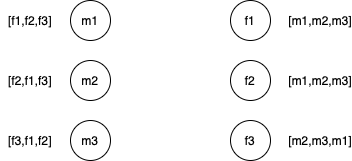
\includegraphics[width=0.4\textwidth ]{GS}
		\caption{An instance of the problem containing the M and W sets and $\forall m \in M, \; \forall w \in W$ a list of preferences for the elements in the opposite set, in increasing order.}
\end{figure}

\begin{figure}[h]
		\centering
		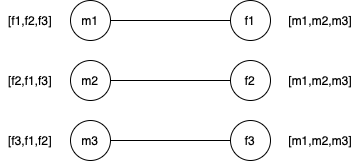
\includegraphics[width=0.4\textwidth ]{GS-Solved}
		\caption{A solution for the instance of the problem, containing only stable pairs.}
\end{figure}


\subsection{The Men-Wimen problem}
The problem about finding the stable matching between a set W and M. Each $w \in W$ rank every $m \in M$ from best to worst, and every $m \in M$ do the same.

\begin{algorithm}[H]
\SetAlgoLined
\small
\KwIn{$M$ set of men, $W$ set of women}
\KwOut{$S$ the set containing all the stable pairs between M and W}
\BlankLine

$S \leftarrow$ set containing all the pairs between M and W.

\BlankLine
\While{$\exists m \in M$ that is free and haven't proposed yet}{
    $w_{i} = m[0] \leftarrow$ first woman in m's list of preference to whom he is not yet proposed \; 
     \If{$w_{i} \; is \; free$}{
     	$S = S \cup p(m,w_{i}) \leftarrow$ create a pair between m and $w_{i}$\;
     }{
      }
      \BlankLine
        \If{$w_{i}$ prefers m to her current partner $m_{i}$}{
        	 $S = S - p(m_{i},w_{i})$\;
     	  $S = S \cup p(m,w_{i})$\;

     }{
      }
      \BlankLine
    
}
\BlankLine

return $S$\;
\caption{proposeAndReject(M, W) :}
\end{algorithm} 

\begin{itemize}
\item Observation 1\\
Every men propose to a women decreasing order of preference, for every women is the opposite. 

\item Observation 2\\
Once a women is matched she never become un-matched, she just change her partner, in increasing order of preference.

\item Observation 3\\
Assuming $|M| = |W|$ then the algorithm has $\mathcal{O}(n^{2})$ complexity.

\item Observation 4\\
The algorithm is very resistant to modifications: example new conditions on engagements.
\end{itemize}

\clearpage

\section{Asymptotic Order of Growth}

\subsection{Brute Force}
For many non-trivial problems, there is a natural brute force search algorithm that checks every possible solution, usually taking $2^{n}$.
\subsection{Polynomial Running Time}
This is the most desirable running time of any algorithm because it scales with ease at the increment of the input size.\\An algorithm can be defined as poly-time if the following property holds:

\[ \exists c > 0, \exists d >0, \; such \; that \; \forall n \in INPUT \; the \; running \; time \; is \; bounded \; by\; cn^{d} \]

We can now give the following definition of efficiency:

\[ An \; algorithm \; is \; efficient \; if \; it \; is \; poly-time.\]

When discussing the running time of a deterministic algorithm is important to take into account the worst-case scenario because, in doing that, the running time is guaranteed $\forall n \in INPUT.$ There are some exception to this rule, when the worst-case scenario is very rare.\\\\
When discussing of probabilistic algorithm we need, instead, to reason upon the expected running time.

\subsection{Big-O Notation}

Assuming we have an algorithm rappresented by the function:
 \[ T(n) = 1.6n^{2} + 3.5n+8\]
 We want a way to express the growing rate in a way that is insensitive to constant factors and low-ordered terms, in fact It can be said that T(n) grows like $\mathcal{O}(n^{2})$.\\

\begin{itemize}
\item The lower bound $\mathcal{O}$\\
We can say that T(n) is $\mathcal{O}{(f(n))}$ if $\exists c > 0, \exists n_{0} \geq 0 / \; T(n) \leq cf(n), \; \forall n \geq n_{0}$

We can give an alternative definition as follow:
 \[ \mathcal{O}{(f(n))} = \lim_{n\to\infty} \frac{T(n)}{F(n)} < \infty\]
 
Graphically:

\begin{figure}[H]
		\centering
		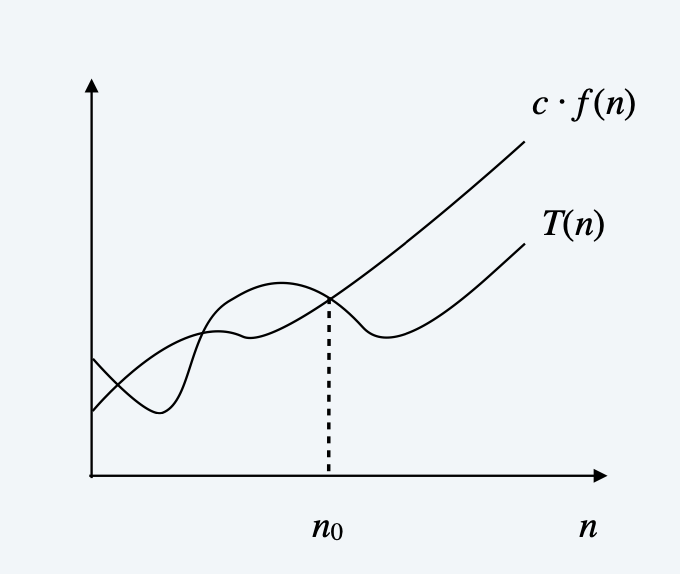
\includegraphics[width=0.4\textwidth ]{on}
\end{figure}

Again, going back to our function: $T(n) = 1.6n^{2} + 3.5n+8$, 
\[ T(n) = n^{3}\]
\[ T(n) = n^{2}\]
\[ T(n) \neq n\]


\item The upper bound $\Omega$ \\
We can say that T(n) is $ \Omega(f(n)) \;if \exists c > 0, \exists n_{0} \geq 0 / \; T(n) \geq cf(n), \; \forall n \geq n_{0}$

Again, going back to our function: $T(n) = 1.6n^{2} + 3.5n+8$, 
\[ T(n) = \Omega(n)\]
since $T(n) \leq pn^{2} \leq pn$.\\


Graphically:

\begin{figure}[H]
		\centering
		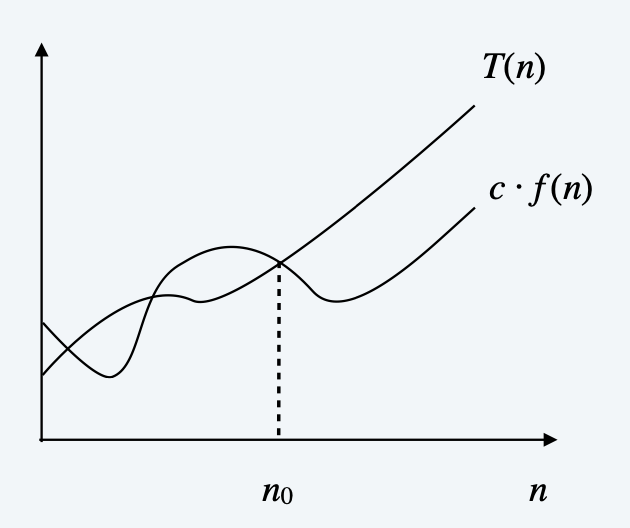
\includegraphics[width=0.4\textwidth ]{omega}
\end{figure}

\item The tight bound $\Theta$ \\
T(n) is $ \Theta(f(n)) \; if \; \exists c_{1} > 0, c_{2}>0 \; and \; \nexists \;n_{0} \; such \; that \; c_{1}f(n) \leq T(n) \leq c_{2} f(n) \; \forall n \geq n_{0}$

Graphically:

\begin{figure}[H]
		\centering
		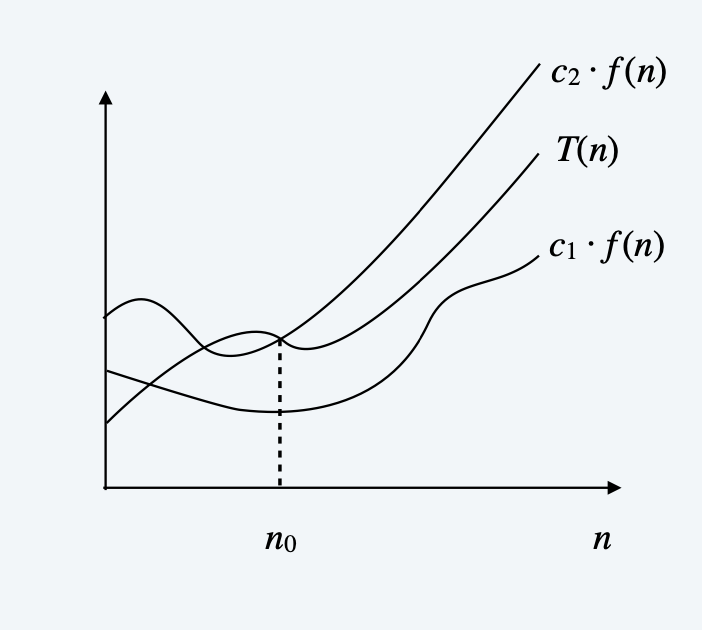
\includegraphics[width=0.4\textwidth ]{tight}
\end{figure}

\item {Usefull Properties}\\\\
Transitivity:
\[ if \; f = \mathcal{O}{(g)} \; and \; g =\mathcal{O}{(h)}, \; then \;f = \mathcal{O}{(h)}\]
\[ if \; f = \Omega{(g)} \; and \; g =\Omega{(h)}, \; then \;f = \Omega{(h)}\]\\\\
Sum of functions:
Supposing that f and g are two functions such that, for some other function h, we have $f = \mathcal{O}{(h)} \; and \;g = \mathcal{O}{(h)}, \; then \; f + g = \mathcal{O}{(h)}.$

\end{itemize}

\subsection{Common Running Times}

\begin{itemize}

\item {Linear $\mathcal{O}{(n)}$}\\\\
The running time is proportional to the input size.\\\\
Example: finding the maximum into an array.

\item {Linearithmic time $\mathcal{O}{(nlogn)}$}\\\\
Very common in divide-and-conquer algorithms, is also the running time of most of the sorting algorithms (ex: MergeSort or HeapSort).\\\\
Note: if an algorithm A execute n times a sorting operation, let's say n=3, and the sorting operation is still the most computational costly operation in the whole algorithm: then A is still $\mathcal{O}{(nlogn)}$ because $3\mathcal{O}{(nlogn)} \simeq \mathcal {O}{(nlogn)}$.

\item {Quadratic time $\mathcal{O}{(n^{2})}$}\\\\
Common when enumerating all pairs of elements, ex: given a list of n points in the plane $(x_{1}, y_{1})$, ..., $(x_{n}, y_{n})$, find the pair that is closest to each other.

\item {Cubic time $\mathcal{O}{(n^{3})}$}\\\\
Example:Set disjointness. Given n sets: $S_{1}, ..., S_{n}$ each of which is a subset of 1, 2, ..., n, is there some pair of these which are disjoint?

\item {Ploynomial time $\mathcal{O}{(n^{k})}$}\\\\
Example:Independent set of size k: Given a graph, are there k nodes such that no two are joined by an edge? The solution is to enumerate all subsets of k nodes.

\item {Exponential time}\\\\
Given a graph, what is maximum cardinality of an independent set? Enumerate all the possible subsets $\Rightarrow \mathcal{O}{(n^{2} 2n)}$

\item {Sublinear time}\\\\
Search in a sorted array. Given a sorted array A of n numbers, is a given number x in the array? $ \Rightarrow \mathcal{O}{(logn)}$ Binary search.

\subsection{Why it Matters}

\begin{figure}[H]
		\centering
		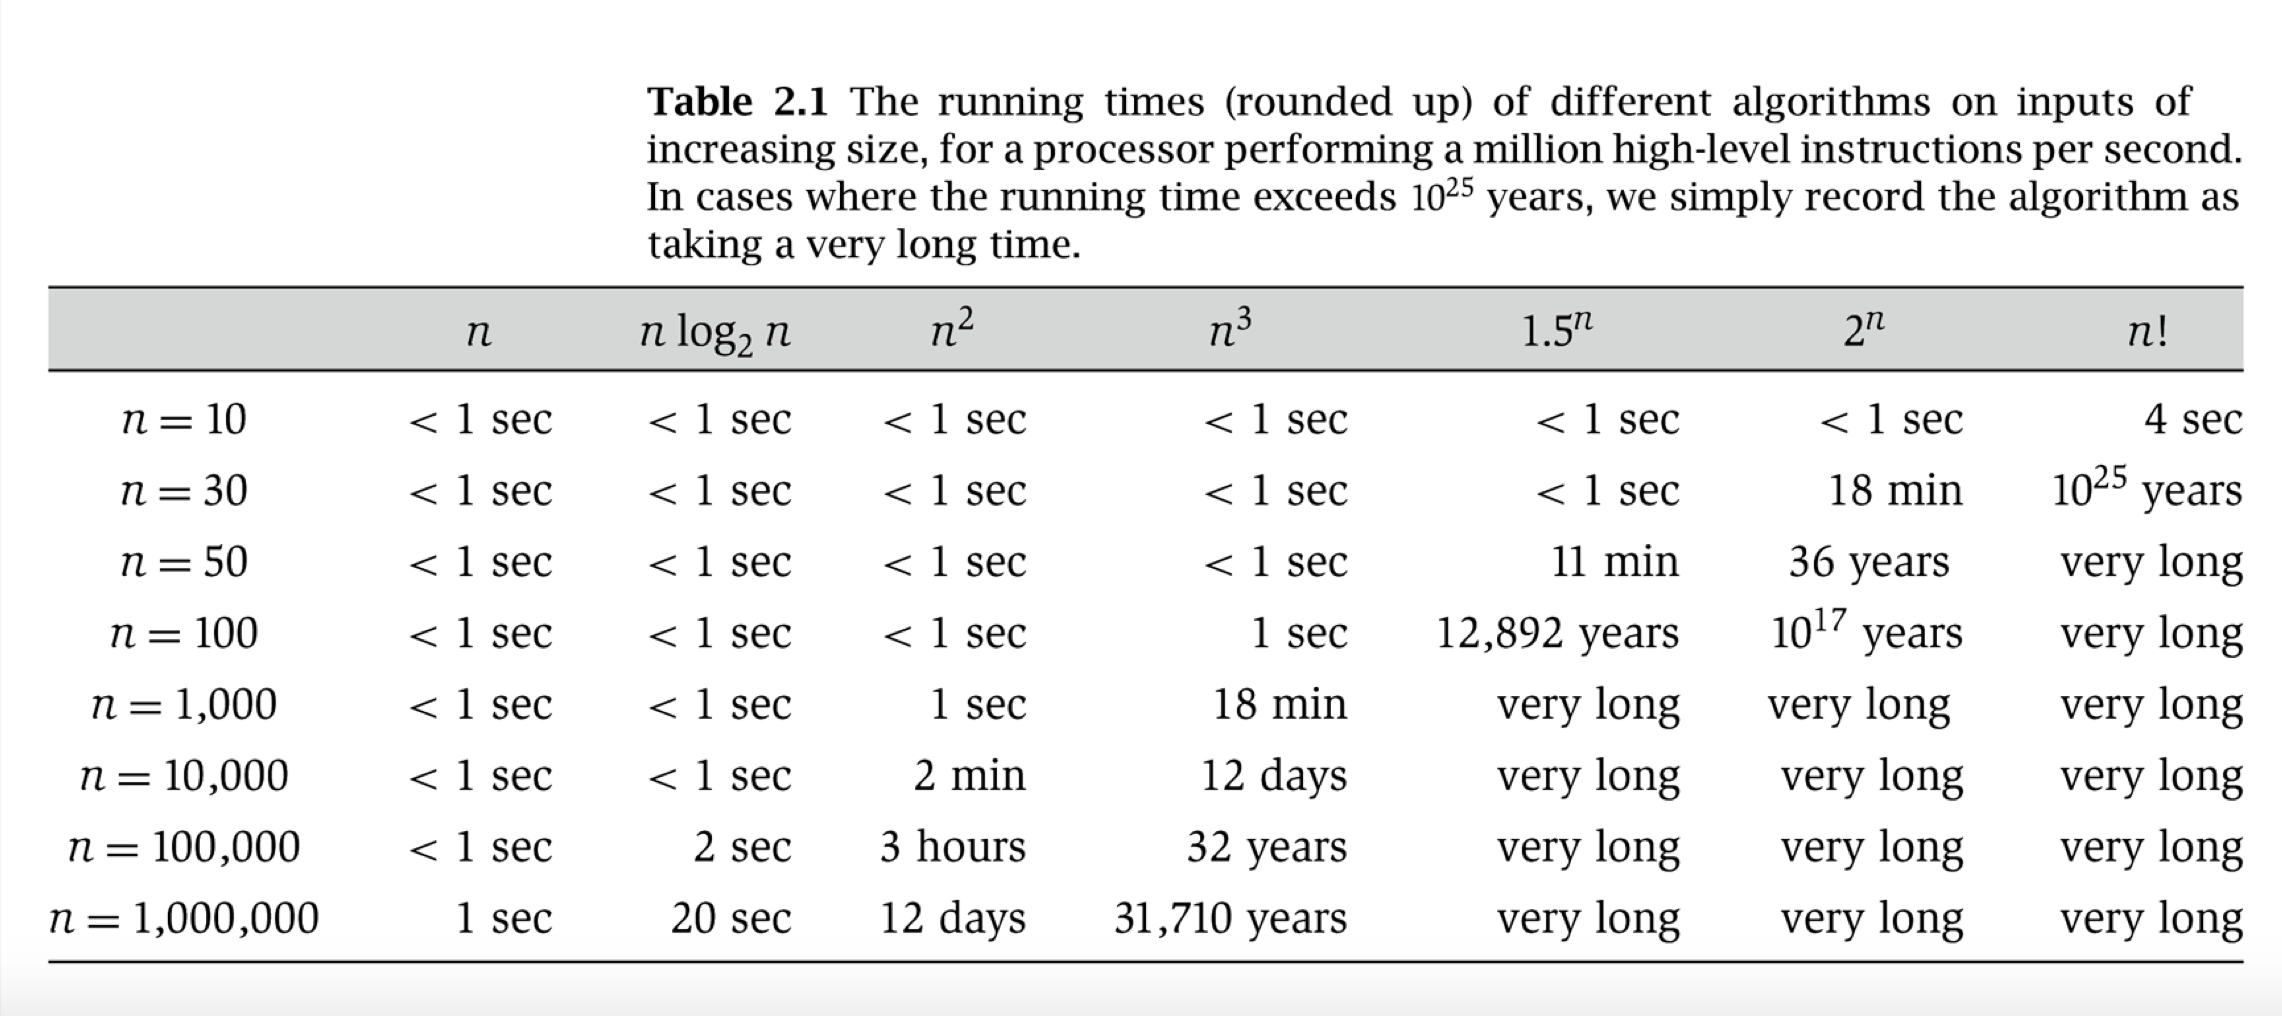
\includegraphics[width=0.7\textwidth ]{running}
		\caption{Comparison of the running times of different complexity algorithms.}
\end{figure}

Notice that, as we distance from the linear complexity, for bigger value of $n \in INPUT$, the execution time goes very high, this is bad: let's just say we want to deploy our non-linear algorithm on a distributed system dealing with a lots of records, as they grows, the system could become unable to process them in a feasible time.

\subsection{The Heap Data Structure}

Is a balanced binary tree  T(V,E) that satisfy the following property, defining with C the set containing all the children of a node $w_{i}$

\[ \forall w_{i} \in V, \forall v_{i} \in C, \; key(w_{i}) \leq key(v_{i})\]

\begin{figure}[H]
		\centering
		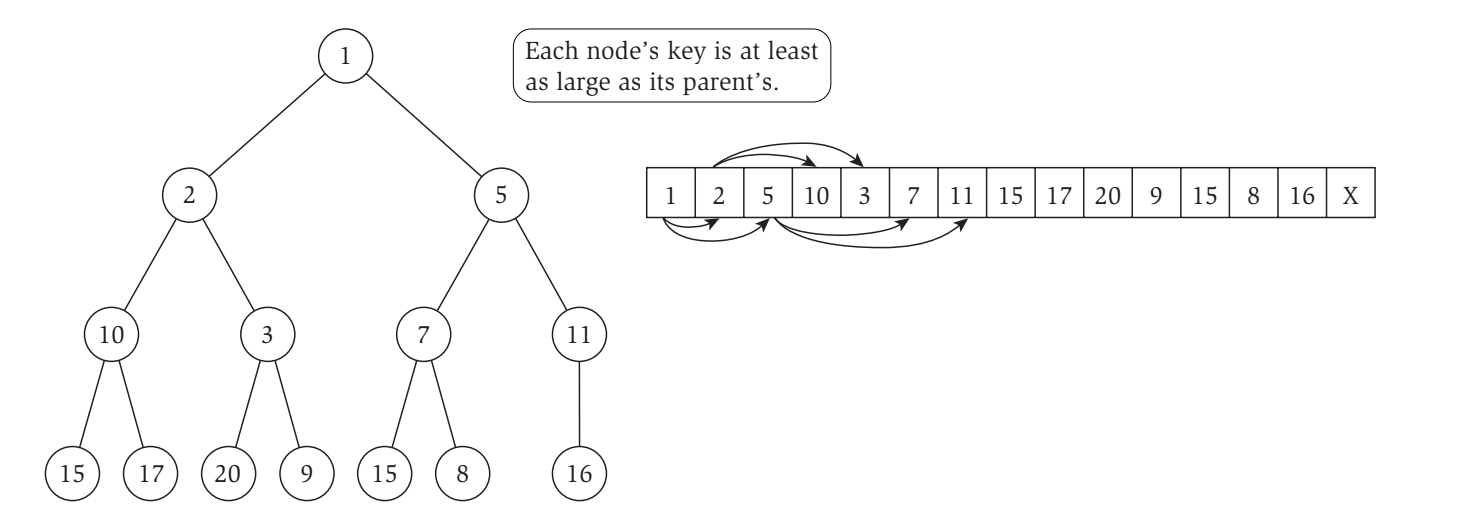
\includegraphics[width=0.7\textwidth ]{heap}
		\caption{An example of heap.}
\end{figure}

This data structure is very helpfull, instead of using an array or a list, here are the complexity of some operations involving the heap structure:

\[ create \; heap =  \mathcal{O}{(n)}\]
\[ insert \; heap =  \mathcal{O}{(logn)}\]
\[find \; min =  \mathcal{O}{(1)}\]
\[delete  =  \mathcal{O}{(logn)}\]

\end{itemize}

\clearpage

\section{Greedy Algorithms}

\emph{Formal definition}: the greedy algorithm "stays ahead" locally: meaning that is better than any other solutions, alternatively we can prove that a greedy algorithm's solution is optimal by transforming the know optimal solution for the problem, into our solution, this method is called "argument exchange".\\\\\emph{Practical definition}: A lot of the time a greedy algorithms involves scanning all the $n \in INPUT$ of the problem, if the current element respect some conditions, then it can be added to the optimal solution returned by the algorithm.

\subsection{The Cashier Problem / Coin changing}

Given a currency with the following values: 1, 5, 10, 25, 100, devise a method to pay amount to customer using fewest number of coins.\\\\
\emph{Example}: 34 dollars, how many coins?\\\\
\emph{Solution}: at each iteration, add coin of the largest value that does not take us past the amount to be paid.

\begin{algorithm}[H]
\SetAlgoLined
\small
\KwIn{$amount$ containing the amount to give back to the client, $C$ set containing all the coins of the current currency. }
\KwOut{$S$ the set containing all the coins to give back to the client}
\BlankLine


$S \leftarrow$ set containing all the coins to give back to the client\;
$total = 0 \leftarrow$ total expressed in the current currency system\;  
$Cs \leftarrow$ set containing all the coins in the currency sorted by increasing values\;

\BlankLine
\While{$total < amount $}{
	  \For{i=Cs.length to 0 }{
	  	\uIf{$total + Cs[i] < amount$}{
		$ total = total + Cs[i]$\;
         	$S = S \cup Cs[i]$\;
		$break;$
     		}
		\uElseIf{$total + Cs[i] = amount$}{
		$S = S \cup Cs[i]$\;
		$ return \; S$\;
     		}{}
	  }  
	  
}
\BlankLine

return $S$\;
\caption{cashierAlgorithm(amount,C):}
\end{algorithm}

\begin{claim}
The cashier algorithm always returns an optimal solution.
\end{claim}
\begin{proof}
The aim of the algorithm is to give as little change as possible (in terms of number of coins), if this is not true, then it must exist a solution $|S^{*}| < |S|$, but the algorithm always give highest compatible coin in the for loop, therefore a contradiction.
\end{proof}\
 
 \subsection{Interval Scheduling}
 
 We have a set J of jobs to execute on a machine and $\forall j \in J \; j=(s_{j},f_{j})$ where s and f are start and finish.Two jobs are compatible if the don't overlap: $\forall j_{i},j_{j} \in C \; f_{i} \geq s_{j} \; or \;vice-versa $.\\
 Once we defined the problem, is just the matter of identifying the best strategy to sort all the jobs in J. Turns out, the best strategy is to sort all the jobs by finishing time, from first to last (for a former proof please check the professor's slide, but the main idea is to prioritize the jobs that release the machine as soon as possible).
 
\begin{algorithm}[H]
\SetAlgoLined
\small
\KwIn{$J$ set containing all the jobs}
\KwOut{$S$ the set containing all the compatible jobs}
\BlankLine

$S \leftarrow$ set containing all the compatible jobs\;
$Js \leftarrow$ set containing all the sorted jobs in increasing order of finishing time $f1 < .... f_{j}$

\BlankLine
\For{i=0 to Js.lenght }{
	  	\If{$J[i].start \geq S.last.finish$}{
			$S = S \cup Js[i]$
		}
		{}
	  }  

\BlankLine

return $S$\;
\caption{earliestFinishingTime(J):}
\end{algorithm}

\begin{claim}
The earliestFinishingTime always return an optimal solution.
\end{claim}
\begin{proof}
Assume this is not true, then it must exist a solution $|S^{*}| > |S|$,containing at least one more compatible job, but the algorithm check every job in J, therefore a contradiction.
\end{proof}\\

\begin{claim}
The complexity of the algorithm is $\mathcal{O}{(nlogn)}$
\end{claim}
\begin{proof}
The for loop costs $\mathcal{O}{(n)}$, while, as stated before, the sorting costs $\mathcal{O}{(nlogn)}$, since $\mathcal{O}{(nlogn)} > \mathcal{O}{(n)}$, the whole algorithm is $\mathcal{O}{(nlogn)}.$
\end{proof}\\

\subsection{Interval Partitioning}
Assuming we have a set of lectures L and, $\forall l \in L ,\; l=(s,f)$ where s and f are start time and finishing time, find the minimum amount of classroom tho schedule all the lectures, so that no two lectures overlap in the same classroom (the definition of overlap is the same as 3.2).

\begin{algorithm}[H]
\SetAlgoLined
\small
\KwIn{$L$ set containing all the lectures}
\KwOut{$S$ set containing the minimum amount of classroom needed}
\BlankLine

$S \leftarrow$ set containing the minimum amount of classroom needed\;
$Ls \leftarrow$ set containing all the sorted lectures in increasing order of starting time $s1 < .... s_{j}$

\BlankLine
\For{i=0 to Ls.lenght }{
	$C = \varnothing$
	
	\uIf{$J[i].start \geq C.last.finish$}{
    	$C = C \cup Ls[i]$\;
  	}
  	\Else{
   	 $S = S \cup C$\;
	 $C = \varnothing$\;
	$C = C \cup Ls[i]$\;
 	 } 
}  

\BlankLine

return $S$\;
\caption{intervalPartitioning(L):}
\end{algorithm}

The number of classrooms needed is more or equal to the depth of $|S|$, that is also the maximum amount of items that contains at any given time.	\\

\begin{claim}
The intervalPartitioning always return an optimal solution.
\end{claim}
\begin{proof}
Same as 3.2, if it exist a better solution $S^{*}$ we would have $|S^{*}| > |S|$ but that is not possible, since the algorithm checks every lecture in the input set. 
\end{proof}\\
 
\begin{claim}
The complexity of the algorithm is $\mathcal{O}{(nlogn)}$
\end{claim}
\begin{proof}
Identical as 3.2.
\end{proof}\\

\subsection{Minimizing The Lateness}
Assuming now we have just one resource that can process just one job at a time, we want to process all possible jobs. For the notation: $\forall j \in J,$ j requires  $t_{j}$ amount  of time to be executed, with a finishing time $f_{j} = s_{j} + t_{j}$, we have also to define a due date $d_{j}$ and finally the lateness of a job as: $max (0,d_{j}-f_{j})$

\begin{algorithm}[H]
\SetAlgoLined
\small
\KwIn{$L$ set containing all the lectures}
\KwOut{$S$ set containing the minimum amount of classroom needed}
\BlankLine

$S \leftarrow$ set containing all the compatible jobs\;
$Js \leftarrow$ set of all jobs sorted by increasing deadline $s1 < .... d_{j}$

\BlankLine
$t = 0 $\;
\For{i=0 to Js.lenght }{
	$s_{i} = t$\;
	$f_{i} = s_{i} + Js[i].finish$\;
	$S = S \cup (s_{i},f_{i})$\;
	$t = t + Js[i].time$\;
}  

\BlankLine

return $S$\;
\caption{earliestDeadLineFirst(J):}
\end{algorithm}

\begin{claim}
EarliestDeadLineFirst algorithm return an optimal solution.
\end{claim}
\begin{proof}
Identical as 3.2 / 3.3.
\end{proof}\\
 
\begin{claim}
The complexity of the algorithm is $\mathcal{O}{(nlogn)}$
\end{claim}
\begin{proof}
Identical as 3.2.
\end{proof}\\

\clearpage

\subsection{Dikstra Algorithm}

\emph{Def}: A path is a sequence of edges which connects a sequence of nodes.\\\\
\emph{Def}: A cycle is a path with no repeated nodes or edges other than the
starting and ending nodes.\\\\
\emph{Shortest Path problem}: Given a digraph G = (V, E), edge lengths $le \geq 0$, source $s \in V$, and destination $t \in V$, find the shortest directed path from s to t.

\begin{figure}[H]
		\centering
		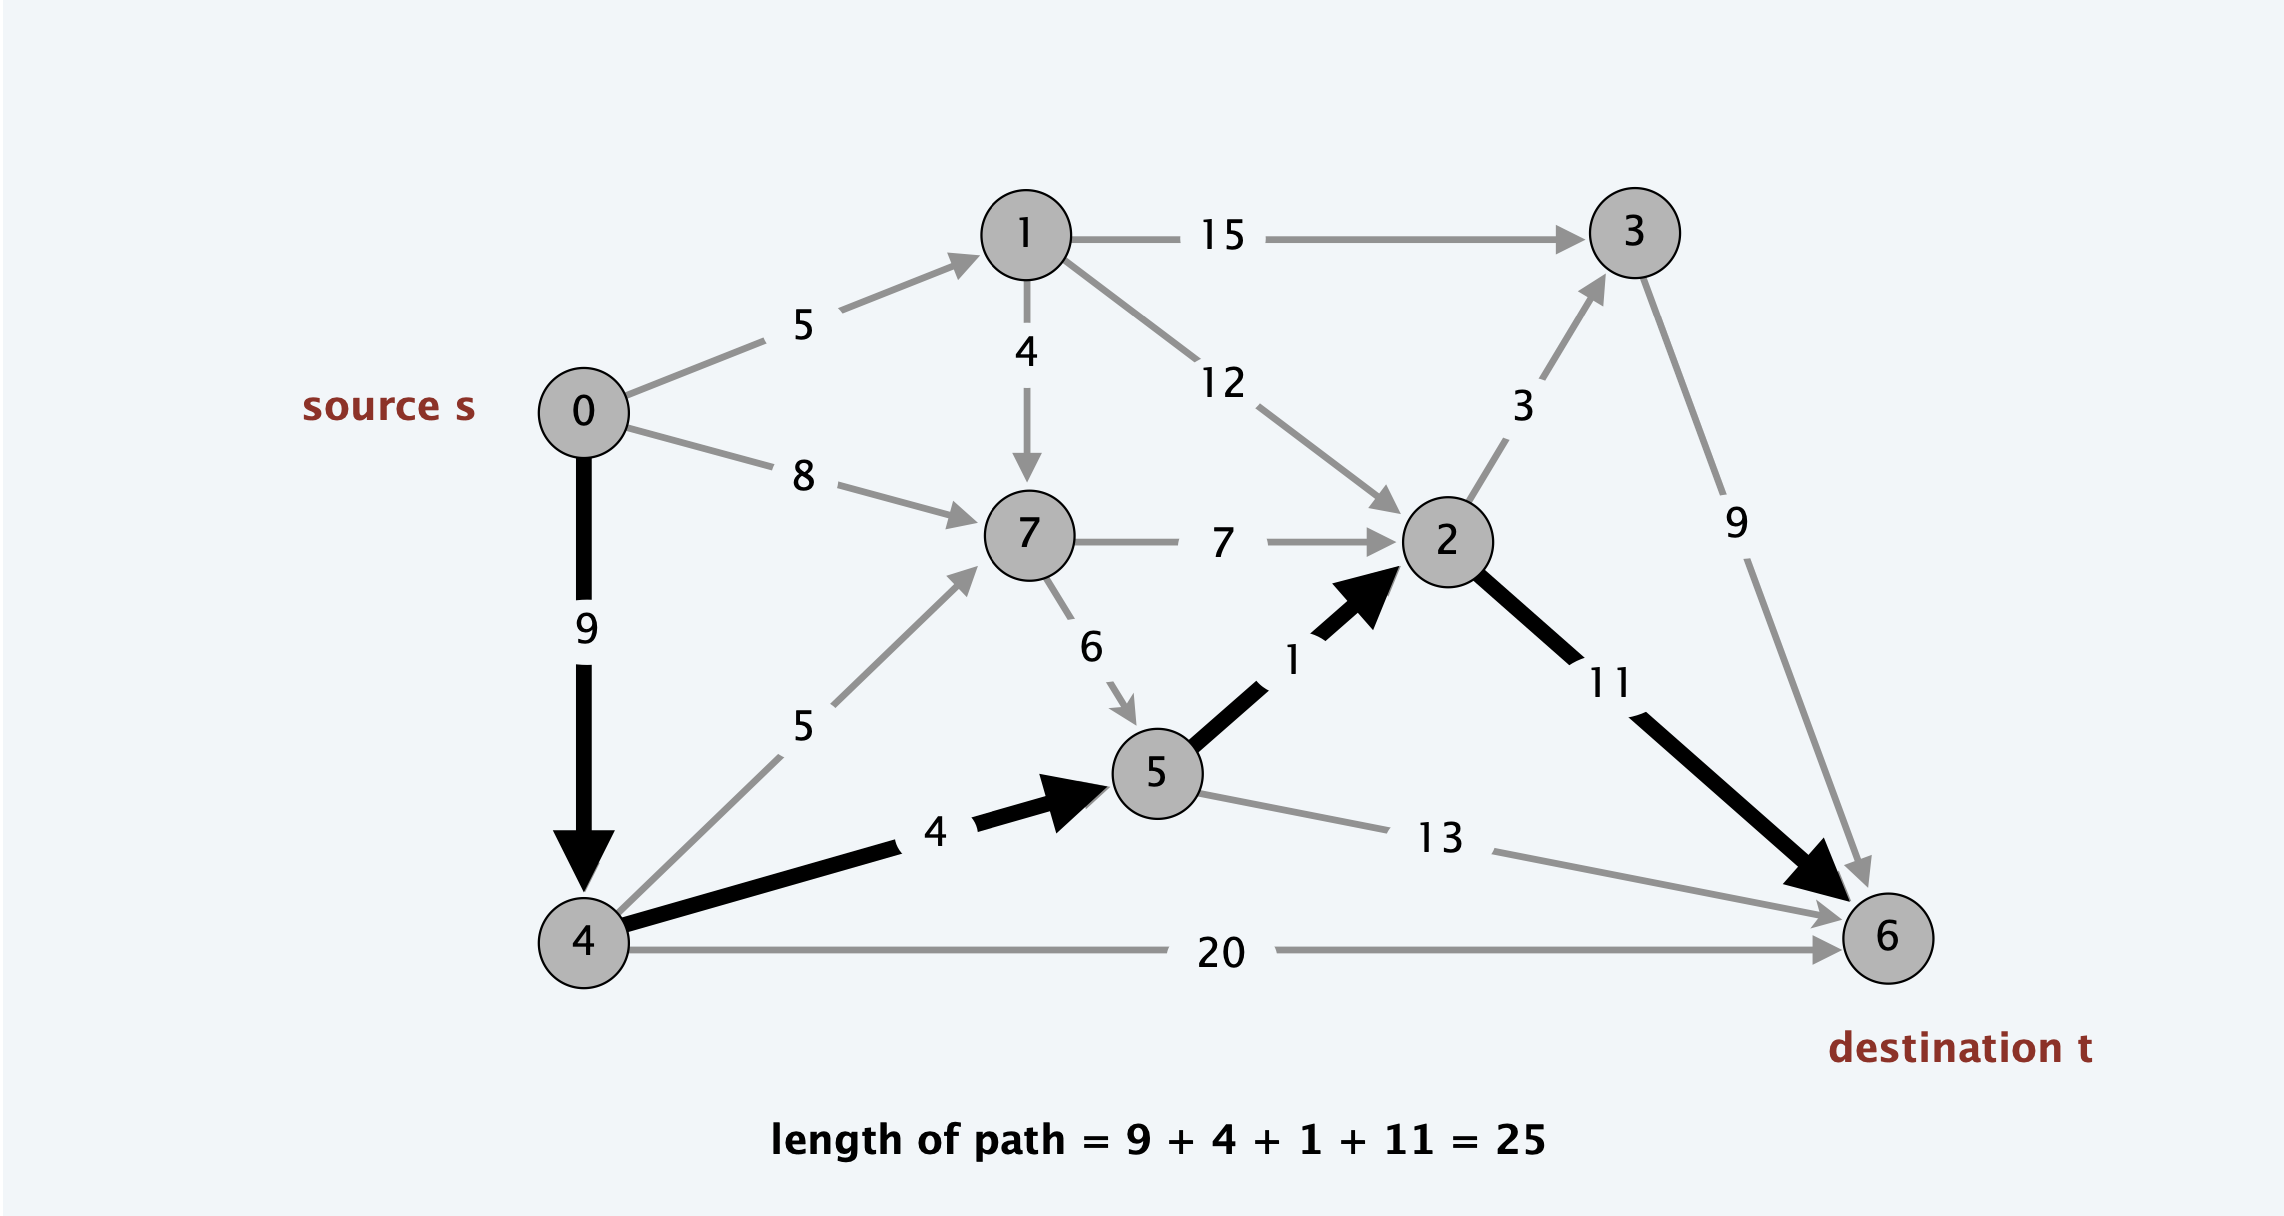
\includegraphics[width=0.8\textwidth ]{dikstra}
		\caption{A solution for the Shortest path problem.}
\end{figure}

\begin{algorithm}[H]
\SetAlgoLined
\small
\KwIn{$G$ set containing all the edges of G, $s$ source of the path}
\KwOut{$S$ set containing all the edges of a shortest path}
\BlankLine

$S \leftarrow$ set containing all the compatible jobs\;
$Q \leftarrow$ priority queue for nodes contained in the unexplored part of G \;
$D \leftarrow$ set of distances from s $\forall \; e \in G$

\BlankLine

$d(s,s) = 0$\;
$D = D \cup d(s,s))$\;

\BlankLine

\For{i=0 to G.lenght }{
	$e_{i} = G[i] \leftarrow$ current edge to check\;
	\uIf{$e_{i} \neq s$}{
	$d(s,e_{i}) = \infty$\;
    	$D = D \cup d(s,e_{i}))$\;
	$Q = Q \cup (e_{i},d(s,e_{i})) \leftarrow$ Insert in queue the current node with key($e_{i}$) = $d(s,e_{i})$\;
  	}
}

\BlankLine

\While{$Q \neq  \emptyset$}{
$u = Q.getMin $\;
$Q = Q - \{u\} $\;
\ForEach {$(u,v) \in G, \; leaving \; u $}{
\uIf{$d(s,v) > d(s,u) + l(u,v)$}{
	$S = S \cup  d(s,u) + l(u,v) $\;
	decrease-key of v to d(u) + l(u, v) in Q.\;
}	
}
}

return $S$\;
\caption{Dikstra(G,s):}
\end{algorithm}

\begin{claim}
The Dikstra Algorithm always return an optimal solution ( $\forall u \in S, \; d(u)$ is the length of the shortest $s\rightarrow u$ path).
\end{claim}
\begin{proof}
Base case: $| S |$ = 1 is easy since S = { s } and d(s) = 0, assume that's true for $| S | > 1$, let v be next node added to S, and let (u, v) be the final edge: the shortest $s\rightarrow u$ path plus (u, v) is an $s\rightarrow v$ path of length $π(v)$. Now consider any $s\rightarrow v$ path P. We show that it is no shorter than $π(v)$. Let (x, y) be the first edge in P that leaves S,and let P' be the subpath to x.\\
P is already too long as soon as it reaches y.
\end{proof}\\

\subsection{Kruskal Algorithm}
Given an undirected, weighted, connected graph G=(V,E) we want to find the all the edges that connects all the nodes with a minimum cost, alternatively we can say that the algorithm finds the minimum spanning tree (MST) of G.\\\\
\emph{Formal definition}: Given an undirected, weighted, connected  graph G = (V, E) with edge costs $c(e)$, an MST is a subset of the edges $T \subseteq E$ such that T is a spanning tree whose sum of edge costs is minimized.

\begin{figure}[H]
		\centering
		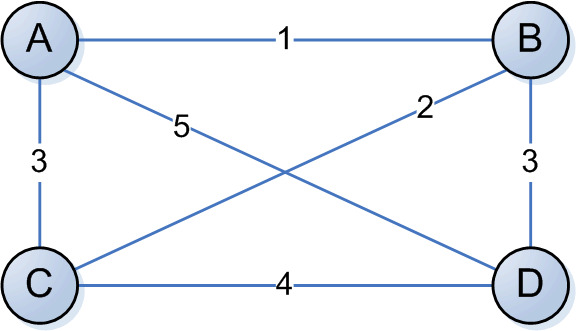
\includegraphics[width=0.4\textwidth ]{kruskal}
		\caption{An instance of the MST problem.}
\end{figure}

\begin{figure}[H]
		\centering
		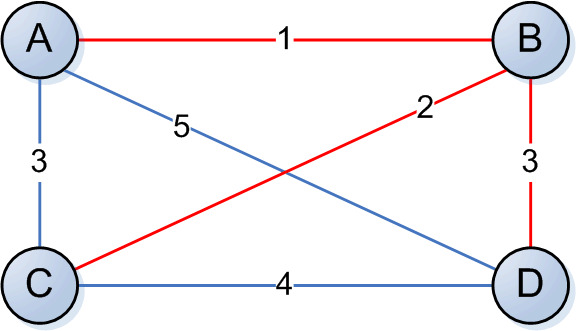
\includegraphics[width=0.4\textwidth ]{kruskal_solved}
		\caption{A solution for the MST problem.}
\end{figure}

\begin{algorithm}[H]
\SetAlgoLined
\small
\KwIn{$G$ set containing all the edges of G}
\KwOut{$S$ set containing all the edges of MST}
\BlankLine

$S \leftarrow$ set containing all the compatible jobs\;
$E \leftarrow$ set of all the edges sorted by increasing weight $c(e)_{1} < .... c(e)_{j}$

\BlankLine

\For{i=0 to G.lenght }{
	$e_{i} = G[i] \leftarrow$ current edge to check\;
	\uIf{$S \cup e_{i} \;is \;not \;a \;loop$}{
    	$S = S \cup e_{i}$ \;
  	}
}  

\BlankLine

return $S$\;
\caption{kruskal(G):}
\end{algorithm}

\begin{claim}
Kruskal algorithm returns an optimal solution.
\end{claim}
\begin{proof}
Identical as 3.2 / 3.3.
\end{proof}\\
 
\begin{claim}
The complexity of the algorithm is $\mathcal{O}{(nlogn)}$
\end{claim}
\begin{proof}
Identical as 3.2.
\end{proof}\\


\end{document}